\section{Evaluation}\label{sec:agg-creds-evaluation}

The performance of the credential system is evaluated via the instantiation over
pairing-friendly groups. The scheme is instantiated using the BLS12-381 pairing
system. The construction relies only on the bilinearity of the pairing system,
and so can easily be instantiated with other pairing systems.

We implement the credential system in Go using the \texttt{gnark-crypto}
library, which provides optimised implementations of group and pairing
operations for BLS12-381~\cite{gnark-crypto}.
We use version 0.21.0 of the library, and implement both $\AAC$ and $\ATS$.
The baseline is Idemix, which is built on BBS+ and uses the same
library~\cite{CCS:CamVan02}. Idemix issues one credential on all $n$ attributes
from one issuer, and presents it with $k$ attributes disclosed. All measurements
are taken on a MacBook Air with an Apple M2 and 16\,GB of RAM, using all eight
cores. Each time is the median of 100 repetitions after ten warm-up calls. The
interquartile range is typically 2\% of the median and never above 6\%, so we
report medians only.

\begin{table}[htbp] \centering
  \begin{tabular}{l l r}
    \toprule
    Algorithm & Party & Time (ms) \\
    \midrule
    $\AACgen$ & & 22.5 \\
    $\AACregister$ & user & 0.149 \\
                   & RA & 0.807 \\
    $\AACissue$ & user & 0.0756 \\
                & issuer & 2.94 \\
    $\AACaggregate$ & user & 0.543 \\
    $\AACpresent$ & user & 20.1 \\
    $\AACverify$ & verifier & 31.1 \\
    \midrule
    $\ATSgen$ & & 0.176 \\
    $\ATSsign$ & & 0.482 \\
    $\ATSrandomise$ & & 0.333 \\
    $\ATSverify$ & & 1.27 \\
    $\ATSaggregate$ & & 0.533 \\
    $\ATSverifyagg$ & & 18.9 \\
    \midrule
    Idemix present & user & 27.0 \\
    Idemix verify & verifier & 11.9 \\
    \bottomrule
  \end{tabular}
  \caption[Aggregate credentials: time of every algorithm]{Time of every
algorithm, for $n = 128$ issuers and $k = 64$ disclosed attributes, medians.
$\AACregister$ and $\AACissue$ are split into the computation of each party. The
$\ATS$ rows sign and aggregate single messages under one tag, with
$\ATSaggregate$ and $\ATSverifyagg$ over $k = 64$ signatures. The Idemix rows
present one credential on $n = 128$ attributes.}
  \label{tab:agg-creds-times}
\end{table}

\begin{table}[htbp] \centering
  \begin{tabular}{l r}
    \toprule
    Object & Size (bytes) \\
    \midrule
    public parameters $\crs$ & 12528 \\
    registration request & 128 \\
    registration credential $\regcred$ & 320 \\
    issuance request & 440 \\
    credential $\cred$ & 192 \\
    aggregate credential $\aggcred$ & 3224 \\
    presentation $\algoproof$ & 10008 \\
    \midrule
    $\ATS$ public key $\pk$ & 96 \\
    $\ATS$ signature $\signature$, single or aggregate & 144 \\
    \midrule
    Idemix presentation & 3034 \\
    \bottomrule
  \end{tabular}
  \caption[Aggregate credentials: sizes]{Size of every object, for $n = 128$
issuers and $k = 64$ disclosed attributes. The Idemix presentation is of one
credential on $n = 128$ attributes.}
  \label{tab:agg-creds-sizes}
\end{table}

\Cref{tab:agg-creds-times,tab:agg-creds-sizes} give the time of every
algorithm and the size of every object at $n = 128$ and $k = 64$. Registration
and issuance depend on neither $n$ nor $k$, and take at most 2.94\,ms for any
party. In registration, the user sends 128 bytes and the registration authority
352 bytes, in three messages in total. In issuance, the user sends 440 bytes and
the issuer 224 bytes, in four messages in total.

\begin{figure}[htbp] \centering
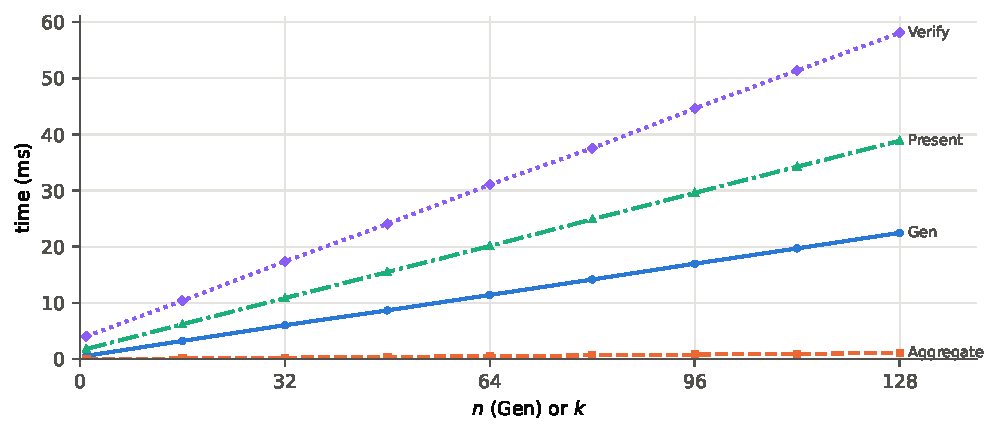
\includegraphics[width=\textwidth]{chapters/04-agg-creds/aggcreds_times.pdf}
\caption[Aggregate credentials: time against $n$ and $k$]{Time of $\AACgen$ against the number of issuers $n$, and of
$\AACaggregate$, $\AACpresent$ and $\AACverify$ against the number of disclosed
attributes $k$. Medians.} \label{fig:agg-creds-times} \end{figure}

\Cref{fig:agg-creds-times,fig:agg-creds-sizes} show how times and sizes change
with $n$ and $k$. Aggregation, presentation and verification grow linearly in
$k$ and do not depend on $n$. The number of issuers $n$ only affects $\AACgen$
and the size of $\crs$.

\begin{figure}[htbp] \centering
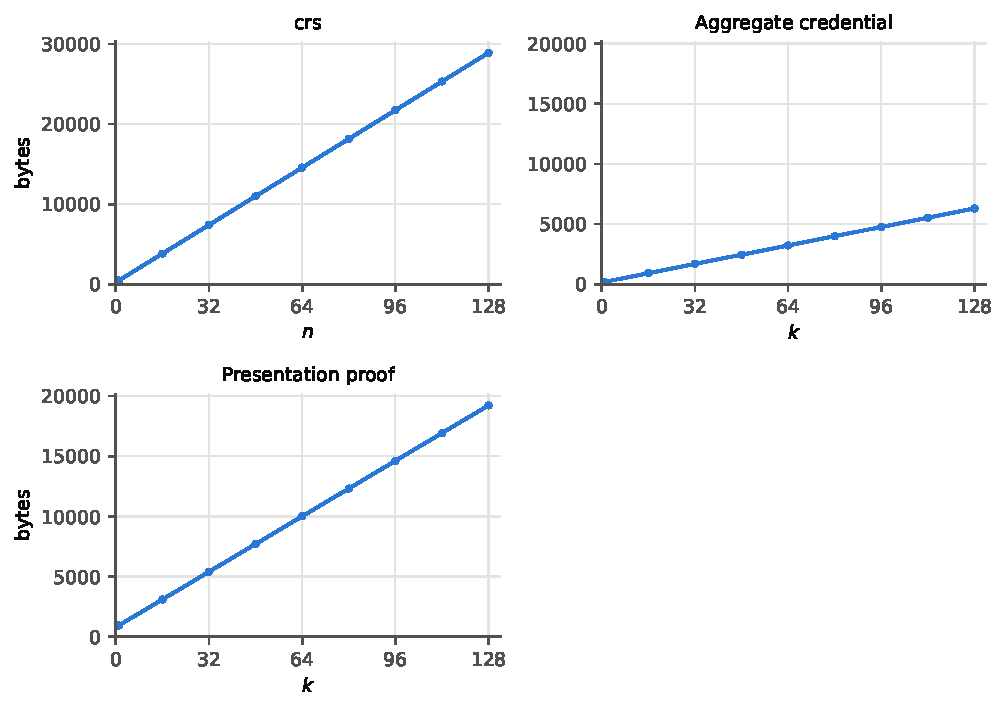
\includegraphics[width=\textwidth]{chapters/04-agg-creds/aggcreds_sizes.pdf}
\caption[Aggregate credentials: sizes against $n$ and $k$]{Size of $\crs$ against the number of issuers $n$, and of the aggregate
credential and the presentation against the number of disclosed attributes
$k$.} \label{fig:agg-creds-sizes} \end{figure}

\begin{figure}[htbp] \centering
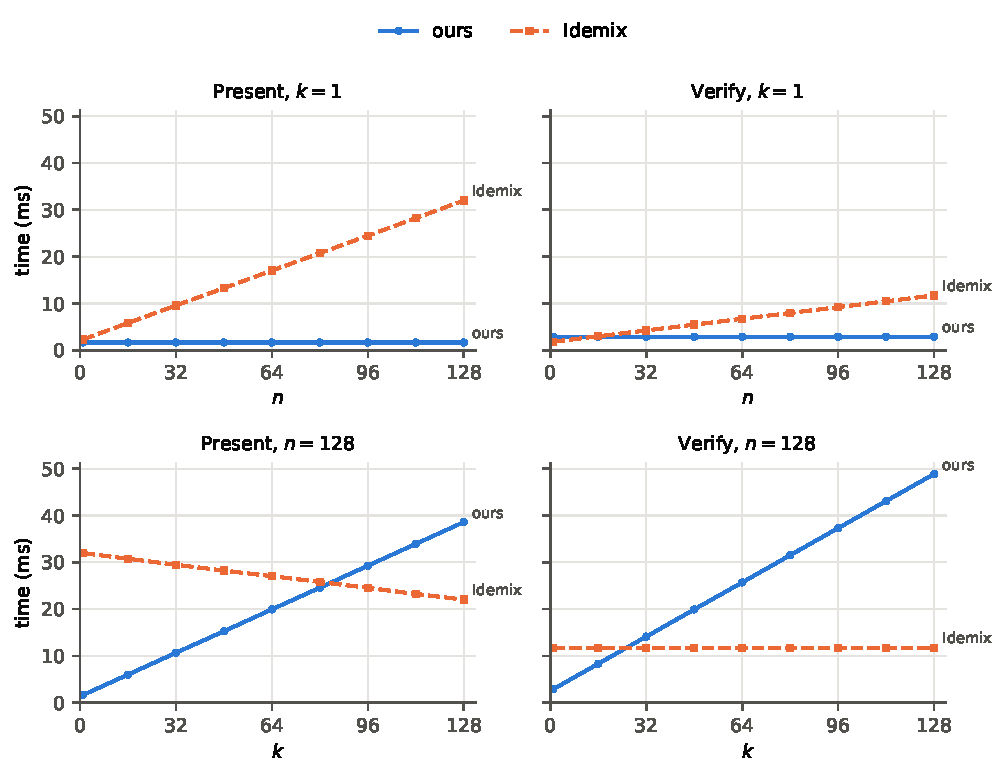
\includegraphics[width=\textwidth]{chapters/04-agg-creds/aggcreds_idemix.pdf}
\caption[Aggregate credentials against Idemix]{Presentation and verification time of our scheme and of Idemix. The top
two panels vary the total number of attributes $n$ with $k = 1$ disclosed, and
the bottom two vary the number of disclosed attributes $k$ with $n = 128$.
Medians.}
\label{fig:agg-creds-idemix} \end{figure}

\Cref{fig:agg-creds-idemix} compares our scheme with Idemix. Idemix proves
knowledge of a signature on all $n$ attributes, so its cost grows with the
attributes held, while ours grows with the attributes disclosed. At $n = 128$
and $k = 1$, presentation takes 1.82\,ms against 31.9\,ms for Idemix, and
verification 4.05\,ms against 11.8\,ms. Idemix verifies faster once more than about
20 attributes are disclosed, but it has one issuer for all attributes, the
setting this chapter avoids.
\begin{outline}
  \item close: costs are low enough for client devices
\end{outline}
